\documentclass{beamer}
%
% Choose how your presentation looks.
%
% For more themes, color themes and font themes, see:
% http://deic.uab.es/~iblanes/beamer_gallery/index_by_theme.html
%
\mode<presentation>
{
  \usetheme{default}      % or try Darmstadt, Madrid, Warsaw, ...
  \usecolortheme{default} % or try albatross, beaver, crane, ...
  \usefonttheme{default}  % or try serif, structurebold, ...
  \setbeamertemplate{footline}[frame number]
  \setbeamertemplate{navigation symbols}{}
  \setbeamertemplate{caption}[numbered]
}

\usepackage[english]{babel}
\usepackage[utf8x]{inputenc}
\usepackage{xcolor}
\usepackage{colortbl}
\usepackage{tikz}
%\usepackage{fancyhdr}

%\pagestyle{fancy}
%\fancyhf{}

%\lfoot{\thepage}
\usetikzlibrary{arrows.meta, shapes.geometric, calc, shadows}


\title[Your Short Title]{EPIC\\\large{Electronic Programmable Intelligent Calculator}}
\author{Florian Weinzerl}
\institute{HTL Hollabrunn}
\date{14.06.2017}

\begin{document}

\section{Titel}

\begin{frame}
  \titlepage
\end{frame}

% Uncomment these lines for an automatically generated outline.
%\begin{frame}{Outline}
%  \tableofcontents
%\end{frame}

\section{Übersicht}

\begin{frame}{Übersicht}

%\vskip 1cm
	
	\begin{itemize}
	  \item Notizen verfassen
	  \item Skizzen erstellen
	  \item Berechnungen durchführen
	  \item Bedienung per Touchscreen
	  \item Speichern von Dateien
	  \item Kompatibilität mit externen Speichermedien
	\end{itemize}

%\begin{block}{Examples}
%Some examples of commonly used commands and %features are included, to help you get started.
%\end{block}

\end{frame}

\section{Praxis}

\subsection{Umsetzung}

\begin{frame}{Umsetzung}

% Commands to include a figure:
%\begin{figure}
%\includegraphics[width=\textwidth]{your-figure's-file-name}
%\caption{\label{fig:your-figure}Caption goes here.}
%\end{figure}

\begin{table}
\centering
\begin{tabular}{l|r}
Hardwareentwicklung & Friesenhengst \\\hline
\rowcolor{blue!25} Mathematik (Theorie) & Weinzerl \\\hline
Software - GUI & Friesenhengst \\\hline
Software - Raspberry Pi, Arduino & Friesenhengst \\\hline
\rowcolor{blue!25} Software - Mathematik & Weinzerl \\\hline
\rowcolor{blue!25} Marketing & Friesenhengst \& Weinzerl
\end{tabular}
%\caption{\label{tab:widgets}An example table.}
\end{table}

\end{frame}


\subsection{Objekt-Struktur}

\begin{frame}{Objekt-Struktur}
\centering
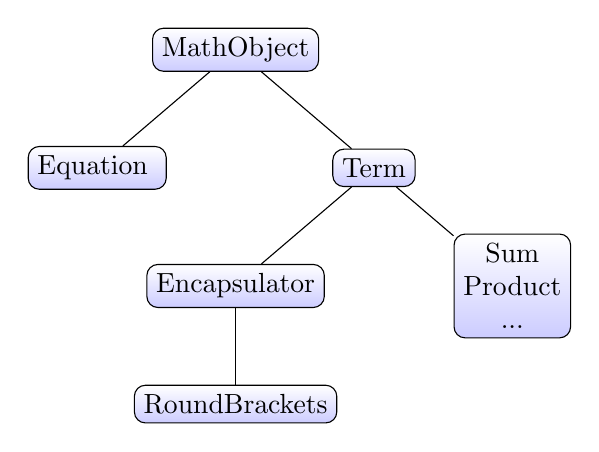
\begin{tikzpicture}[sibling distance=10em,
every node/.style = {shape=rectangle, rounded corners,
	draw, align=center,
	top color=white, bottom color=blue!20}]]
\node {MathObject}
child { node{ Equation } }
child { node {Term}
	child { node{Encapsulator}
		child { node{RoundBrackets} } }
	child { node {Sum\\ Product\\ ...} }
};
\end{tikzpicture}

\end{frame}

\subsection{Implementierung}

\begin{frame}{Implementierung}
	\centering
	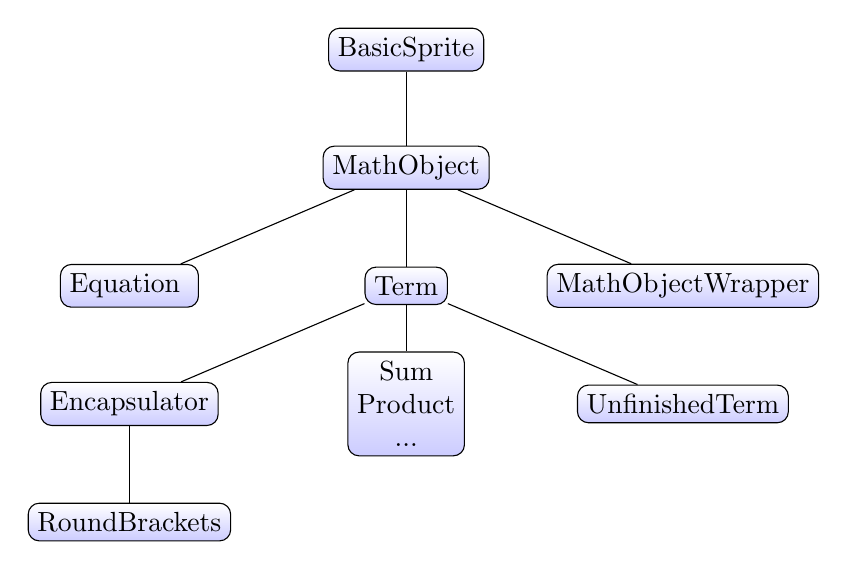
\begin{tikzpicture}[sibling distance=10em,
	every node/.style = {shape=rectangle, rounded corners,
		draw, align=center,
		top color=white, bottom color=blue!20}]]
	\node {BasicSprite}
	child { node{MathObject}
		child { node{ Equation } }
		child { node {Term}
			child { node{Encapsulator}
				child { node{RoundBrackets} } }
			child { node {Sum\\ Product\\ ...} }
			child { node {UnfinishedTerm} }
		}
		child { node {MathObjectWrapper} } };
	\end{tikzpicture}
	
\end{frame}

\subsection{Benutzer-Eingabe}
\begin{frame}{Benutzer-Eingabe}
	\begin{itemize}
		\item \textit{abstract}-Klasse Parser
		\item rekursive parse-Methode
		\item offset beachten!
		\item globales Parser-Verzeichnis
		\item UnfinishedTerm ruft Parser auf
	\end{itemize}
\end{frame}

\subsection{Mathematik}
\begin{frame}{Mathematik-Zusatz}
	\begin{itemize}
		\item Gleichungssysteme lösen nach Gauß
		\item Nullstellen finden (Newton): \[ x_{n+1}=x_{n}-{\frac {f(x_{n})}{f'(x_{n})}}\]
		\item Polynomisierung (Taylor): \[f(x)=\sum _{n=0}^{\infty }{\frac {f^{(n)}(a)}{n!}}(x-a)^{n}\]
	\end{itemize}
\end{frame}

\subsection{Marketing1}

\begin{frame}{Marketing}

\begin{block}{Analyse des Käuferverhaltens}
	\begin{itemize}
		\item	Wer kauft? \hspace{1.1cm} $\rightarrow$ \hspace{0.5cm} Träger der Kaufentscheidung
		\item	Was? \hspace{2cm} $\rightarrow$ \hspace{0.5cm} Kaufobjekte
		\item	Warum? \hspace{1.52cm} $\rightarrow$ \hspace{0.5cm} Kaufmotive
	\end{itemize}
\end{block}

\end{frame}
\subsection{Marketing2}
\begin{frame}{Marketing}

\begin{block}{Analyse des Käuferverhaltens}
	\begin{itemize}
		\item	Wie? \hspace{2.1cm} $\rightarrow$ \hspace{0.5cm} Kaufentscheidungsprozess
		\item	Wie viel? \hspace{1.45cm} $\rightarrow$ \hspace{0.5cm} Kaufmenge
		\item	Wann? \hspace{1.8cm} $\rightarrow$ \hspace{0.5cm} Kaufzeitpunkt, -häufigkeit
		\item	Wo bzw. bei wem?  $\rightarrow$ \hspace{0.5cm} Einkaufsstätten, Lieferantenwahl
	\end{itemize}
\end{block}

\end{frame}

\subsection{Demo}
\begin{frame}{Demo}
	
\end{frame}

\end{document}